\section{Lecture 32}
\textbf{Today}
\begin{enumerate}[1.]
    \item Quiz \#3 - Nov. 29$^\text{th}$, 7-8pm [Sec. 9.2-9.7 except 9.3 (Markov Chains)]
    \item Cat exercise
    \item Indicator variables
\end{enumerate}
\textbf{Cat Exercise}

How many cats would you need to have for a $ 0.95 $ probability
that the average height is within 1cm of the true average? 

\textbf{Solution.}
Let $ X $ be the height of the cat.
\[ X \thicksim N(24,1.5^2) \]
(finding the middle 0.95, tails are $ 0.025 $ each; in the table we look
for $ 0.975 $)

\begin{center}
    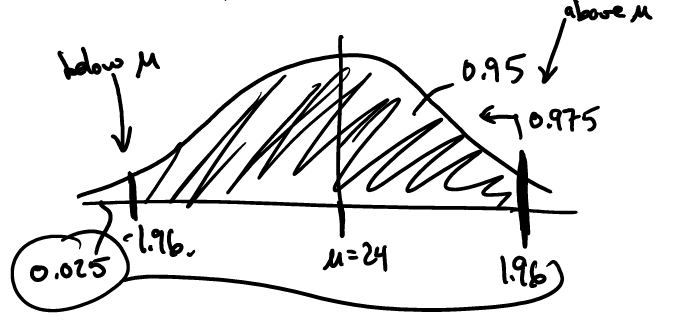
\includegraphics{catscurve.png}
\end{center}
\begin{align*}
    P\left(\left|\bar{X}-24\right|<1\right)=0.95
\end{align*}
\[ P(0.975)=1.96 \]
\[ Z=\pm 1.96\implies Z=\frac{\bar{X}-\mu}{\nicefrac{\sigma}{\sqrt{n}}}
\implies 1.96=\frac{25-24}{\nicefrac{1.5}{\sqrt{n}}} \]
$ n=8.64=9 $

\subsection{Indicator Variables (9.7)}
A tool you can use to evaluate more complicated distributions.

\begin{defbox}
    \subsection{Definition (Indicator Variable)}
    An \emph{indicator variable} (Bernoulli variables)
    \[ I_A=
    \begin{cases}
        1,\,\text{if $A$ occurs}\\
        0,\,\text{if $A$ does not occur}
    \end{cases} \]
\end{defbox}

$ E(I_A)=1P(A)+0(1-P(A))=P(A)$

$ E(I_A^2)=1^2P(A)+0^2(1-P(A))=P(A) $

$ Var(I_A)=E(I_A^2)-(E(I_A))^2=P(A)-(P(A))^2=P(A)(1-P(A)) $

\[ I_B= \begin{cases}
    1,\,\text{if $B$ occurs}\\
    0,\,\text{if $B$ does not occur}
\end{cases} \]
$ Cov(I_A,I_B) $

\begin{center}
    \begin{tabular}{| *{3}{>{\centering\arraybackslash}p{2cm} |}}
        \hline
        $I_B\backslash I_A$ & 0 & 1\\
        \hline
        0 & 0 & 0\\
        \hline
        1 & 0 & 1\\
        \hline
    \end{tabular}
\end{center}
\[ I_AI_B=
\begin{cases}
    \left.\begin{aligned}0\\
    0\\
    0\end{aligned}\right\}\text{otherwise}\\
    1,\,\text{if $A$ and $B$ occur}
\end{cases} \]

$E(A)=P(A)$

$ E(B)=P(B) $

$ E(I_AI_B)=P(AB) $

\[ Cov(I_A,I_B)=P(AB)-P(A)P(B) \]

\begin{remark}
    If $ A $ and $ B $ are independent, $ I_A $ and $ I_B $ will be uncorrelated.
\end{remark}

1. Let $ X \thicksim \bin(n,p) $
use indicator variables to find $ \mu $ and $ \sigma^2 $

Let
\[ X_i=
\begin{cases}
    1,\,\text{if trial $ i $ is a success}\\
    0,\,\text{if trial $ j $ is a failure}
\end{cases} \]
then $ X =X_1+X_2+\cdots+X_n$.

$ E(X_i)=p $

$ E(X)=E(\sum\limits_{i=1}^{n} X_i)=\sum\limits_{i=1}^{n} E(X_i)=np=\mu $

$ Var(X)=\sum\limits_{i=1}^{n} Var(X_i)=np(1-p)=\sigma^2 $

2. $ X \thicksim \hyp(N,r,n) $; reminder: 
($ N $ trials, $ r $ S's, $ n $ selections)
Let
\[X_i=\begin{cases}
    1,\,\text{if object $ i $ is a success (S)}\\
    0,\,\text{if object $ j $ is a failure (F)}
\end{cases} \]

$ E(X_i)=P(\text{select object is an S})=\nicefrac{r}{N} $
[from $E(I_A)=P(A)$]

$ Var(X_i)=\nicefrac{r}{N} (1-\nicefrac{r}{N} ) $
[from $ Var(I_A)=P(A)-(1-P(A)) $]

\begin{align*}
    Cov(X_i,X_j)
    &=P(\text{objects $ i $ and $ j $ are S's})-
    \left(\frac{r}{N}\right)\left(\frac{r}{N}\right)\\
    &=\frac{\binom{r}{2}}{\binom{N}{2}}-\left(\frac{r}{N}\right)^2\\
    &=\frac{r(r-1)}{N(N-1)} -\frac{r^2}{N^2}\\
    &=-\frac{r(N-r)}{N^2(N-1)}<0  
\end{align*}
$ X=\sum\limits_{i=1}^{n} X_i\implies E(X)=\sum\limits_{i=1}^{n} \nicefrac{r}{N} =
\nicefrac{nr}{N} $

$ Var(X)=\sum\limits_{i=1}^{n} Var(X_i)+2 \sum\limits_{i<j} Cov(X_i,X_j)  $

where $ Var(X) $ comes from properties in 9.5, the first term has $ n $ terms,
the second term has $ \binom{n}{2} $ terms.
\[=\frac{nr}{N} \left(1-\frac{r}{N}\right)+2\left(\frac{n(n-1)}{2}\right)
\left(-\frac{r(N-r)}{N^2(N-1)}\right)=\frac{nr}{N} \left(1-\frac{r}{N}\right)
\left(\frac{N-n}{N-1}\right) \]
where $ \frac{nr}{N} \left(1-\frac{r}{N}\right)$ is $\bin(n,\nicefrac{r}{N}) $
and $ \left(\frac{N-n}{N-1}\right) $ reduces variance because sampling without replacement.

\textbf{Example}

$ N $ messages come to a server which randomly gives one message to each
intended recipient. Find the mean and variance of the \# of correctly delivered
messages.

\textbf{Solution.}

Let
\[ X_i=
\begin{cases}
    1,\,\text{if msg $ i $ is correct}\\
    0,\,\text{otherwise}
\end{cases} \]
then $ X=\sum\limits_{i=1}^{N}X_i $

$
\left.\begin{aligned}
E(X_i)=P(\text{msg $ i $ is correct})=\frac{1}{N}\\
Var(X_i)=\frac{1}{N}\left( 1-\frac{1}{N} \right)
\end{aligned}\right\}\text{properties of indicator variables}
$
\begin{align*}
    E(X_iX_j)
    &=P(\text{$ i $ correct})P(\text{$ j $ correct}|\text{$ i $ correct})\\
    &=\frac{1}{N}\frac{1}{N-1}\\
    &=\frac{1}{N(N-1)}
\end{align*}
$ Cov(X_i,X_j)=\frac{1}{N(N-1)}-\left( \frac{1}{N} \right)^2=
\frac{1}{N^2(N-1)} >0$

$ E(X)=\sum\limits_{i=1}^{N} E(X_i)=\sum\limits_{i=1}^{N}\frac{1}{N}
=N\frac{1}{N}=1 $

$ Var(X)=1\rightarrow\text{ for Diana} $
